% !TeX root = ../../thesis.tex
\chapter{Nucleation probability assessment - a phase field methodology}
\section{Introduction}
This chapter develops a methodology to obtain insight about the nucleation barrier from the equilibrium shapes of particles with anisotropic interface energy obtained by phase field simulation. The used model represents wetting of a plane by a crystal and combines the features developed by the author: the inclination dependence of interface energy, volume conservation using the fictitious concentration field approach and the general Neumann boundary conditions to control the interface inclination at the domain boundary. 

Advantage of the method is that it does not a-priori assume any shape, it is thus in principle usable for non-analytic cases, where the solution is not known.

The below procedure assumes a 2D particle sitting on top of a line, the contact angles on the left and right are known. It is assumed that the environment surrounding the particle is liquid and the particle-liquid energy is anisotropic. The contact angles are determined using the Young's equation. 

The following sections describe how the phase field result can be used to bring insight about the nucleation barrier using scaling of simulation domain, which is a kind of post-processing of the results. 

\section{Simulated system}
Principle of the method is in utilizing the fact, that in the simulated geometry, the total energy of the system is in fact the particle-liquid interface energy. 

The critical nucleation barrier is total energy change upon insertion of the critical nucleus. That is such nucleus, which just balances the bulk and interface energy contributions. 

The phase field simulation provides the interface-energy-minimizing shape for the input contact angles

The simulated system geometry is sketched in Figure~\ref{fig_sketch_domain_scaling_PF}. A two-phase system of aparticle in a liquid was described by two phase field variables in Moelans' model, one representing the liquid parent phase ($\eta_1$) and the second ($\eta_2$) representing the particle (possibly with anisotropic interface energy). The bottom domain boundary then represents the substrate and the interface inclination in the two contact points is controlled by the boundary condition as indicated in the figure.
\begin{figure}
	\centering
	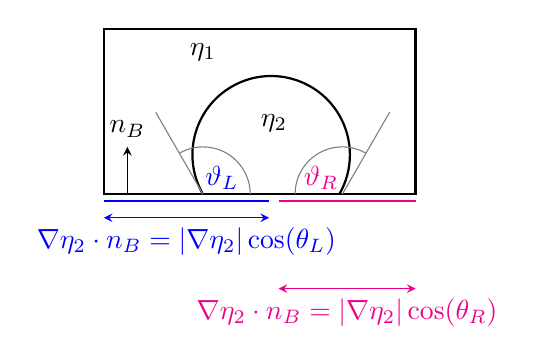
\begin{tikzpicture}[scale=3]
		\draw[thick] (-0.22,0) rectangle (1.1,.7); 
		\draw[thick] (1/5,0) arc (210:-30:1/3);
		\draw[blue] (0.28,0.07) node {$\vartheta_L$};
		\draw[magenta] (0.7,0.07) node {$\vartheta_R$};
		\draw[gray] (0.59,0) arc (180:60:0.2);
		\draw[gray] (0.4,0) arc (0:120:0.2);
		\draw[gray] (1/5,0) -- ++(120:0.4);
		\draw[gray] (0.79,0) -- ++(60:0.4);
		
		\draw (0.2,0.6) node {$\eta_1$};
		\draw (0.5,0.3) node {$\eta_2$};
		
		\draw[-stealth] (-0.12,0) -- ++(0,0.2) node[above] {$\bm{n_B}$};
		\draw[blue,stealth-stealth] (-0.22,-0.1) -- node[below,midway]{$\nabla\eta_2\cdot\bm{n_B}= |\nabla\eta_2|\cos(\theta_L)$}  (0.48,-0.1); 
		\draw[blue,thick] (-0.22,-0.03) -- (0.48,-0.03); 
		\draw[magenta,thick] (1.1,-0.03) -- (0.52,-0.03); 
		\draw[magenta, stealth-stealth] (1.1,-0.4) -- node[below,midway]{$\nabla\eta_2\cdot\bm{n_B}= |\nabla\eta_2|\cos(\theta_R)$} (0.52,-0.4);
	\end{tikzpicture}
	\caption{Sketch of the geometry in the phase-filed simulations used in the domain scaling methodology for nucleation barrier assessment. The symbols $\vartheta_L,\vartheta_R$ denote tangent angles in the contact points and $\theta_L,\theta_R$ the normal ones. The intervals on the bottom domain boundary with the different interface inclination imposed are indicated (note that $\eta_1$ has analogous boundary conditions which must be consistent).}
	\label{fig_sketch_domain_scaling_PF}
\end{figure}

Volume conservation was assured using the fictitious concentration field. 

\section{Some fundamentals}
In 2D, the Gibbs free energy difference upon a nucleus insertion in the system is due to competition between area and line energy contributions (see also Figure \ref{fig_nucl_barrier}b). Be $A_{hom}$ the nucleus area and its interface be described by a parametric curve $\mathcal{C}$. In the isotropic case, $\mathcal{C}$ is a circle and the interfacial contribution is simply $\sigma L$, where $L=2\pi R$ is the interface length and $\sigma$ the isotropic specific interface energy. The Gibbs free energy difference of a free nucleus is then (with $\Delta G_A$ being supersaturation)
\begin{align}
	\Delta G_{hom} &= -\Delta G_A A_{hom} + \sigma L \\
	&= (-\Delta G_A R^2 + 2R\sigma)\pi \,,
\end{align}
which implies the critical radius
\begin{equation} \label{eq_crit_radius_2D}
	R_c = \frac{\sigma}{\Delta G_A}
\end{equation}
and critical nucleation barrier
\begin{equation} 
	(\Delta G_c^*)_{hom} = \hat{A}_{hom}\frac{\sigma^2}{\Delta G_A}\,,
\end{equation}
where the non-dimensional nucleus area is $\hat{A}_{hom}=A_{hom}/R^2=\pi$.

In heterogeneous nucleation, the shape factor $S(\theta)=A_{het}/A_{hom}$ has equal role as in the 3D space, implying
\begin{equation}\label{eq_DG_het_2D}
	\Delta G_{het} = S(\theta)\Delta G_{hom}
\end{equation}
similarly as for the nucleation barrier
\begin{equation}\label{eq_nucl_barr_het_2D}
	(\Delta G_c^*)_{het} = S(\theta)(\Delta G_c^*)_{hom}\,.
\end{equation}

When the interface energy is inclination-dependent $\sigma(\theta)=\sigma_0 f(\theta)$, the interface energy contribution is a line integral $\int_\mathcal{C} \sigma(\theta) \mathrm{d}l$, which can be expressed in analogy with the 3D case~[Mariaux2010] as ($X_0$ being the generalized radius of the Wulff shape with area $A_{hom}^{ani}$)
\begin{equation}
	\int_\mathcal{C} \sigma(\theta) \mathrm{d}l = \frac{2\sigma_0}{X_0}A_{hom}^{ani} \,,    
\end{equation}
which eventually allows to write the Gibbs free energy difference of a free nucleus
\begin{equation}\label{eq_DG_hom_aniso}
	\Delta G_{hom}^{ani} = (-\Delta G_A X_0^2 + 2\sigma_0 X_0)\hat{A}_{hom}^{ani} 
\end{equation}
and further its nucleation barrier
\begin{equation} 
	(\Delta G_c^*)_{hom} = \hat{A}_{hom}^{ani}\frac{2\sigma^2}{\Delta G_A}\,.
\end{equation}
In the heterogeneous anisotropic nucleation the difference in Gibbs free energy is like in equation~\eqref{eq_DG_het_2D}, having $\Delta G_{hom}^{ani}$ as in~\eqref{eq_DG_hom_aniso} and the nucleation barrier like in~\eqref{eq_nucl_barr_het_2D}, only with modified shape factor correspondingly to the Wulff shape.
\begin{figure}
	\begin{tikzpicture}
		\newcommand{\sig}{1}
		\newcommand{\dGv}{\sig}
		\newcommand{\barr}{0.5*\sig^2/\dGv}
		\newcommand{\xlim}{2.5}
		\begin{axis}[
			small,
			clip mode=individual,
			xlabel={radius $R/R_c$},
			ytick={0},
			ylabel={$\Delta G$ (a.u.)},
			ylabel near ticks,
			ymin=-1.2,
			ymax=1.7,
			legend entries={$\approx- R^2$,$\approx R$,$\Delta G$},
			legend pos = north east,
			ymajorgrids = true
			]
			
			\addplot[blue,domain=0:\xlim,samples=50] {-\dGv*x^2/2};
			\addplot[red,domain=0:\xlim,samples=50] {\sig*x};
			\addplot[black,domain=0:\xlim,samples=50] {-\dGv*x^2/2+\sig*x};
			
			\draw[stealth-stealth] (axis cs:1,0) -- (axis cs:1,\barr/2)  node [left] {$\Delta G_c^*$} -- (axis cs:1,\barr);
			
			\draw (rel axis cs: -0.15,1) node [left,inner sep=0] {a)};
%			\draw (rel axis cs: -0.15,1) node [left,inner sep=0] {a)};
		\end{axis}
	\end{tikzpicture}
\end{figure}
	


\section{Methodology - domain scaling}
The critical nucleation barrier is the maximal possible energy change attributed to insertion a nucleus of a particular shape, interface energy and in the present supersaturation (bulk driving force in general). In 
The Gibbs free energy change upon a nucleus insertion in 2D reads 


\section{Implementation of general Neumann BC}
The Appendix~\ref{ch_numerical_implementation} contains the necessary modifications to the finite-difference algorithm when implementing the general Neumann boundary conditions. Eventually, the changes affected all the finite difference operators (standing in place of unidirectional derivatives and laplacian), but only in the parts of the matrices, which interact with the domain boundary.

	\subsection{Tilted straight line}
	The implementation of general Neumann boundary conditions controlling the inclination angle at the domain boundary was validated in simulations sketched in Figure~\ref{fig_sketch_tilted_plane_validation}. A slightly different approach had to be taken in the case with isotropic and anisotropic interface energy, as described below.
	
	In the case with isotropic interface energy, the initial condition for the simulation was a tilted line, which was inclined under different angle $\vartheta_{init}$ than the imposed inclination angle $\vartheta$. The simulation ran until the total energy converged (i.e. until the change in energy per time step was smaller than a threshold). The final state was expected to be a line aligned under the target angle $\vartheta$. From linear fit of the final phase field contour, the resulting inclination angle was read out. A range of angles between 15\textdegree-165\textdegree was probed, and the results were plotted in Figure~\ref{fig_tilted_plane_validation_results}a. As can be seen, a perfect match was achieved.
	
	When validating the same with inclination-dependent interface energy, the methodology had to be modified slightly: the straight line was placed in its imposed position already in the initial condition, i.e. $\vartheta_{init}=\vartheta$. That was because once any curvature appeared in the straight line (which happened when the interface was forced to move by the boundary conditions), it began deforming and there remained no straight line. To assure that the tilted line be the equilibrium state of the system, the anisotropy function was always rotated so that the target inclination angle $\vartheta$ corresponded to the minimal interface energy. Only then the straight line could be immobile and the general Neumann BC could be validated in the same way like with the isotropic interface energy, i.e. simulation until energy convergence and linear fit of the contour. The target angle was observed very accurately in this case as well, as can be seen in Figure~\ref{fig_tilted_plane_validation_results}b.
	\begin{figure}
		\centering
		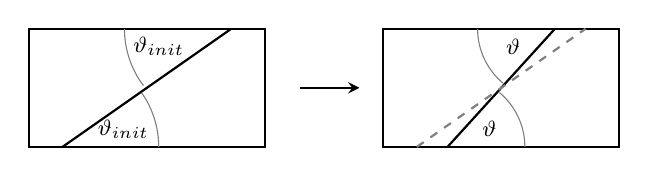
\begin{tikzpicture}[scale=1.5]
			\draw[thick] (0,0) rectangle (2,1);
			\draw[thick] (1-0.5/0.7,0) -- (1+0.5/0.7,1);
			\draw (0.8,0.15) node {\footnotesize$\vartheta_{init}$};
			\draw (1.1,0.85) node {\footnotesize$\vartheta_{init}$};
			\draw[gray] (0.81,1) arc (180:217:0.8);
			\draw[gray] (1.1,0) arc (0:35:0.8);
			
			\draw[thick,-stealth] (2.3,0.5) -- (2.8,0.5);
			
			\draw[thick] (3,0) rectangle (5,1);
			\draw[thick] (4-0.5/1.1,0) -- (4+0.5/1.1,1);
			\draw[dashed,gray,thick] (4-0.5/0.7,0) -- (4+0.5/0.7,1);
			\draw (3.9,0.15) node {\footnotesize$\vartheta$};
			\draw (4.1,0.85) node {\footnotesize$\vartheta$};
			\draw[gray] (3.8,1) arc (180:230:0.6);
			\draw[gray] (4.2,0) arc (0:50:0.6);
		\end{tikzpicture}
		\caption{Validation of the general NBC for control of the inclination angle at the boundary - tilted line simulations (isotropic interface energy). In the simulations with inclination-dependent interface energy there was $\vartheta_{init}=\vartheta$}
		\label{fig_sketch_tilted_plane_validation}
	\end{figure}
	\begin{figure}
		\centering
		\begin{tikzpicture}
			\node[below right, inner sep=0] (L) at (0,0) {
				\includegraphics[width=0.48\textwidth]{validation_iso_specBC_planar.png}};
			\node[below right, inner sep=0] (R) at (L.north east) {
				\includegraphics[width=0.48\textwidth]{validation_aniso_specBC_planar_final.png}};
				
			\draw[above ] (L.north west) node {(a)};
			\draw[above ] (R.north west) node {(b)};
		\end{tikzpicture}
		\caption{Results of tilted plane validation. In a) the result with isotropic interface, in b) with anisotropic one. }
		\label{fig_tilted_plane_validation_results}
	\end{figure}
		
	\subsection{Examples}



\section{Proof-of-concept application}
%%%%%%%%%%%%%%%%%%%%%%%%%%%%%%%%%%%%%%%%%%%%%%%%%%
% Keep the following \cleardoublepage at the end of this file, 
% otherwise \includeonly includes empty pages.
\cleardoublepage

% vim: tw=70 nocindent expandtab foldmethod=marker foldmarker={{{}{,}{}}}
